%!TEX root = ../thesis.tex
\chapter{Design \& Implementation}

	Development of a graphical user interface for libmapper creates a unique challenge. Obviously such an interface is a practical tool, and should function as such, yet it also must work in concert with DMIs which are inherently designed for creative use. For the purposes of this project, the assumed solution to this innate paradox is to provide the user with multiple independent modes of control.  libmapper itself is an extremely flexible API that makes few assumptions as to the network of devices and signals or how they are mapped. It is thus fitting that a GUI for libmapper would be equally as flexible. In lieu of a single perfect solution for network visualization and interactivity, providing users with various independent solutions provided a good compromise.

	Work began with the webmapper interface described in section \ref{sub:webmapper}. An MVC structure was built around the code in order to make the program more extensible and allow for the easy integration of multiple views. Missing features from Maxmapper are incorporated into the main view mode, known as the ``list'' view. That interface has been extended in various ways, taking advantage of the new code base. Two new view modes, the ``grid'' and ``hive'', both designed by Jonathan Wilansky at IDMIL, are integrated into the main GUI. Finally, the code has been compiled together as a standalone application, ready for wide distribution.

%%%%%%%%%%%%%%%%%%%%%%%%%%%%%%%%%%%%%%%%%%%%%%%%%%%%%%%%%%%%%%%%%%%%%%%%%%%%%%%%%%%%%%%%%%%%%%%%%%%%%%%%%%%%%%%%%%%%%%%%%%%%%%%%%%%%%%%%%%%%%%%%%%%%%%%%%%%%%%%%%%%%%%%%%%%%%%%%%%%%%%%%%%%%%%%%%%%%%%%%%%%%%%%%%%%%%%%%%%%%%%%%%%%%%%%%%%%%%%%%%%%%%%%%%%%%%%%%%%
\section{Development of a Flexible System} % (fold)
\label{sec:development_of_a_flexible_system}

Prior GUIs for libmapper have been successfully used for some time, but all have failed to become a standard for the same reason: they cannot accommodate all possible use-cases of libmapper. List based views like the Max/MSP GUI and webmapper cannot show hierarchies while the cluster view implemented in vizmapper can be overly cumbersome for interaction with simple networks. Especially with so much work already completed on prior GUIs, it is more suitable to integrate different approaches into a single GUI than to begin work on some new, hopefully superior approach that would likely prove to be flawed like all that came before it. 

Interface integration is accomplished through an extremely simple approach: a drop-down menu is added to the upper left corner of the interface. Options on this menu represent different visualization modes available to the user. By selecting a new visualization mode the GUI drastically changes it appearance, replacing nearly every visual element in the display.
	%Needs to be adaptable, show any metadata

	\subsection{MVC architecture} % (fold)
	\label{sec:mvc_architecture}

Because a modular design is desired, the Model-View-Controller (MVC) metaphor for structuring software applications \cite{MVC_krasnerpope} is used as a general framework for structuring the application. In fact, the whole scale swapping in and out of independent visual modes would be straightforward implementation of MVC. Unfortunately, the \url{libmapper} $\rightarrow$ \url{python monitor} $\rightarrow$ \url{browser} implementation is slightly more complicated than as imagined by \citeANP{MVC_krasnerpope}. Figure \ref{fig:mapper_network} can be contrasted with (TODO). A few layers of abstraction are added to take into account the monitor, the network itself and control features independent to the view (see section \ref{sec:top_toolbar}), but the general MVC architecture is maintained.

\begin{figure}[!ht]
\centering
	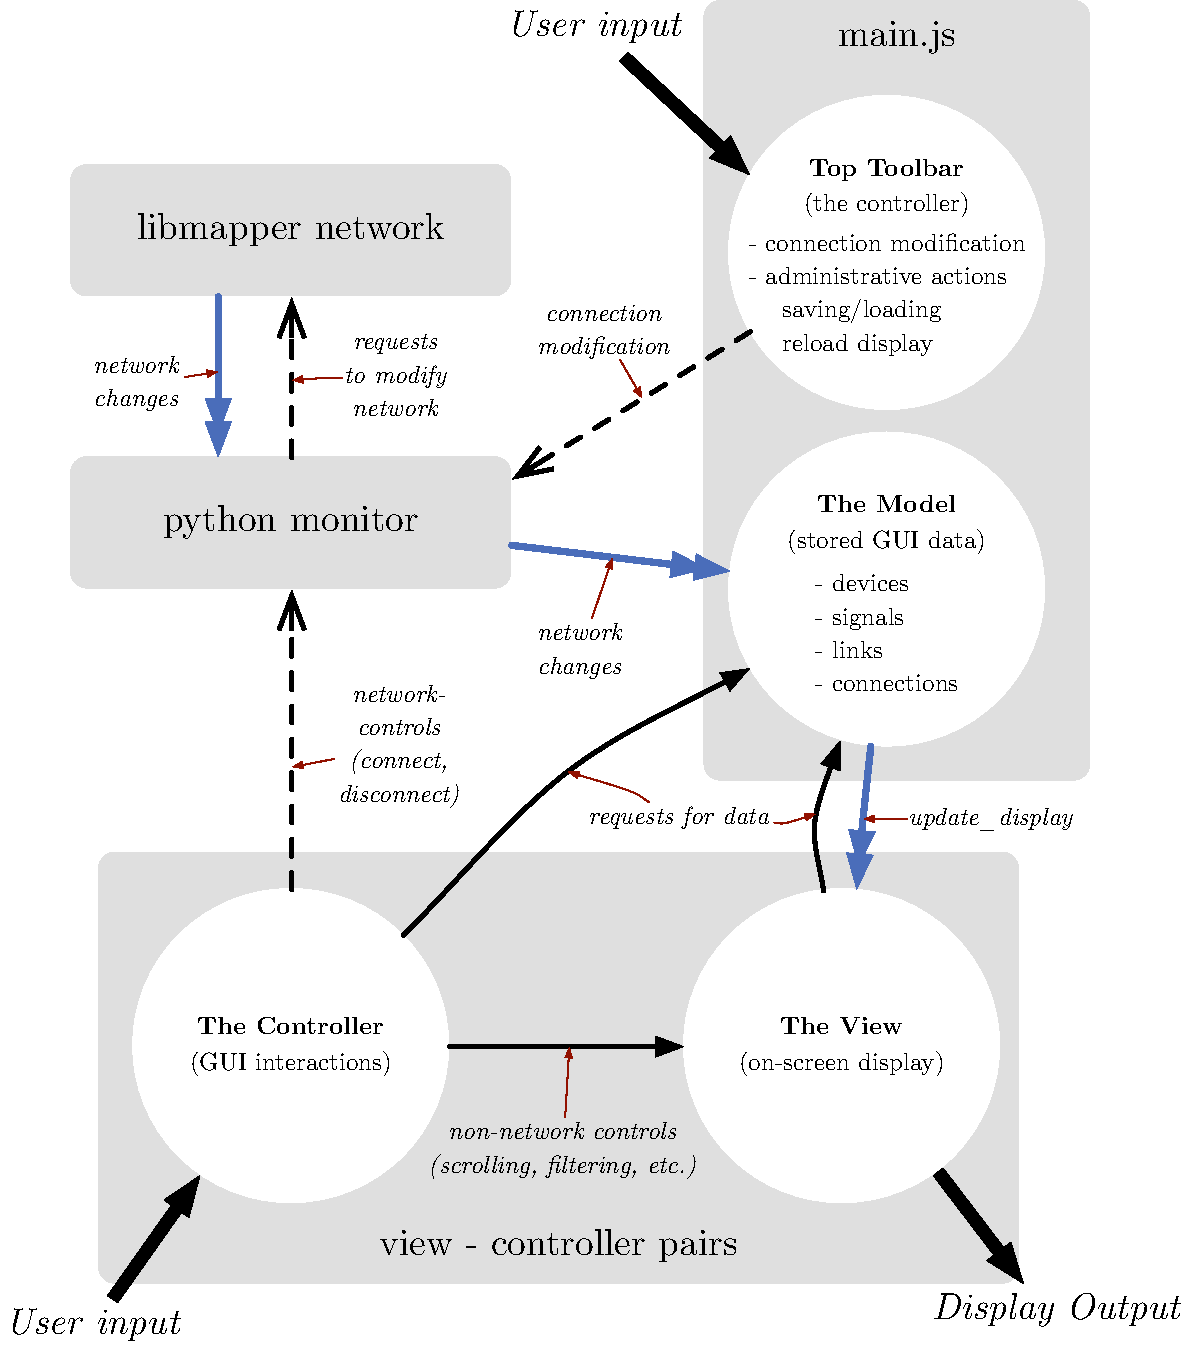
\includegraphics[width=0.9\textwidth]{figures/mapper_network2}
\caption{MVC hierarchy for the GUI and libmapper, blue arrows show propagation of network changes, dashed arrows denote messages requesting a network change.}
\label{fig:mapper_network}
\end{figure}


		\subsubsection{Independent communication}

First and foremost, it is essential that data on the screen should reflect data on the network. This is not entirely straightforward, as asynchronous messages are constantly being sent from the GUI to libmapper and vice versa. In a truly distributed system, data on the libmapper network will be constantly changing as other users add devices and modify mappings. As can be seen in figure \ref{fig:mapper_network}, the actual libmapper network, the displayed data and user interaction are very insulated from one another. For example, a user command to link two devices (in this case \url{source.1} and \url{dest.1}), the following message will be sent to the python monitors:

\url{ {"cmd":"link","args":["/source.1","/dest.1"]} }

Meaning: a linking command is sent to \url{source.1} and \url{dest.1} (the command itself is a python dictionary). After this, the display will not do anything, as the display has not yet been notified of the link. The monitor then relays this message to the network, using libmapper specific syntax. If the link is successful, the monitor receives notice, and sends a message to the main JavaScript file (main.js):

\url{("new_link", {"src_name": "/source.1", "dest_name": "/dest.1"}) }

This states that a new link has been formed between the source device \url{source.1} and the destination device \url{dest.1}. Only then does the GUI respond to the change on the network. Signal data itself is not available to the GUI in any way, as libmapper networks are designed to prevent this kind of bandwidth clutter \shortcite{new_libmapper}.

		\subsubsection{The model}

The model consists of an abstract copy of the network, residing on the local machine. Independent views can consult these data, but cannot directly modify it. Messages from the python monitor announce new links, modifications to connections, or any other changes on the network. All of these changes are recorded and reflected in the model. The model itself consists of four data structures.

\begin{itemize}
 	\item \url{model.devices}: Storage of all present devices and device metadata.
 	\item \url{model.links}: A record of all links presently on the network.
 	\item \url{model.signals}: Keeps track of signals on the network, but only whichever signals are currently visible in the GUI. This is done to save bandwidth and processing power. View-controller pairs keep track of which devices are currently being viewed, and can ask for their child signals. 
 	\item \url{model.connections}: All connections and connection metadata between signals currently in the model.
 \end{itemize} 

It is possible that previously viewed signals will persist in the model, but they and their connections will not be updated upon change.

		\subsubsection{View-controller pairs}

All interaction handlers\footnote{Response to mouse clicks and certain keypresses.} and visualizations are stored in modular, view-controller pairs, as recommended by \citeN{MVC_krasnerpope}. Each view controller pair corresponds with a single view mode. Pairs can have any combination of UI handlers and visual features, but must have the following four functions that are called by the main file on which the model is stored:

\begin{itemize}
	\item \url{view.initialize()}: Calls upon the view to create its visual elements and add 
	\item \url{view.get_focused_devices()}: Returns whichever devices are currently visible in the view. This is used for populating the signal and connection data structures.
	\item \url{view.cleanup()}: Causes the controller to remove all interaction handlers.
	\item \url{view.update_display()}: Called whenever the model changes. The view is not made explicit aware of \emph{what} has changed, only that a change has occurs. In each view mode, this call causes visual features to be cleared and re-drawn, much like a screen refreshes. Though this creates more processor overhead (see section \ref{sec:testing_program_responsiveness}), it allows for much greater flexibility in designing new views.
\end{itemize}

	% subsection mvc_architecture (end)

	\subsection{Top toolbar} % (fold)
	\label{sec:top_toolbar}

One crucial way that the program departs traditional MVC is that the controller is broken up into two distinct parts. An extra ``user-input'' and controller section sits at the top-right corner of figure \ref{fig:mapper_network}, as a child of \url{main.js}.  It also would be possible to think of this as a separate view-controller pair, running constantly and simultaneously with the others, but since it is a part of the main JavaScript file, network visualization is more straightforward when it is thought of as an isolated controller.

Certain tasks and information providing structures are sensible to include across visualization modes. In light of this, a static toolbar is presented at the top of the GUI. This toolbar contains all administrative controls and connection modification fields.

\begin{figure}[!ht]
\centering
	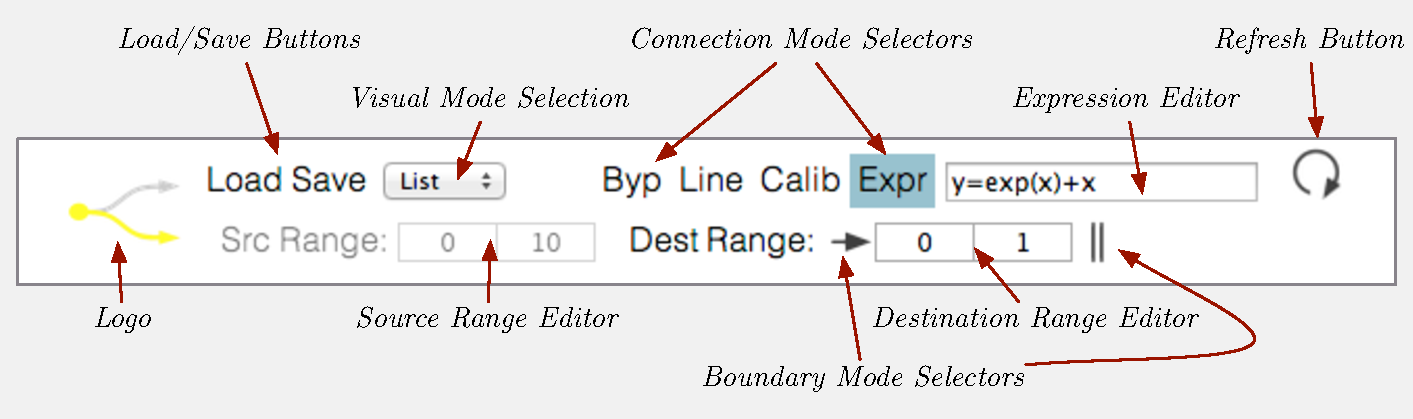
\includegraphics[width=1\textwidth]{figures/top_toolbar}
\caption{The upper toolbar}
\label{fig:toolbar}
\end{figure}

\begin{itemize}
	\item \textbf{Administrative controls}
	\begin{itemize}
		\item\emph{Load/Save buttons}: These elements respond to clicks and save and load mappings, as discussed in section \ref{sec:saving_and_loading}.
		\item\emph{Visual mode selection}: A drop-down menu containing all possible view modes (at the writing of this thesis: List, Grid and Hive), allowing the user to select between them.
		\item\emph{Refresh Button}: When clicked, all data residing on the GUI is erased and re-gathered. This is useful if the monitor somehow desynchronizes with the network.
	\end{itemize}

	\item \textbf{Connection modification}
	\begin{itemize}
		\item\emph{Connection mode selectors}: If a single connection is selected within the GUI, this array of buttons allows the user to choose between the available connection modes.
		\item\emph{Expression editor}: Here the user inputs a custom expression, if in ``Expr'' mode, in other modes this field displays the connection's expression but is not editable.
		\item\emph{Source range editor}: These two numbers reflect the maximum and minimum values of the input signal, is only editable in the ``Line'' connection mode.
		\item\emph{Destination range editor}: Same as above but for the destination signal. Due to boundary conditions these fields are useful in all modes.
		\item\emph{Boundary mode selectors}: Two buttons that cycle through five boundary modes for both the maximum and minimum destination value. A graphic exists to represent each mode.
	\end{itemize}
\end{itemize}

All interface features not present in the top toolbar are part of the current visualization mode and are placed into a ``container'' element below, occupying the remainder of the window.

	% subsection top_toolbar (end)

The file and communication structure described in this section allows for quick modification and extension of the interface. Developers can program new visual modes relatively easily, in comparison to prior GUIs. Hopefully this will eventually lead to a GUI with many useful view modes that can accommodate nearly every use-case for libmapper.

% section development_of_a_flexible_system (end)

%%%%%%%%%%%%%%%%%%%%%%%%%%%%%%%%%%%%%%%%%%%%%%%%%%%%%%%%%%%%%%%%%%%%%%%%%%%%%%%%%%%%%%%%%%%%%%%%%%%%%%%%%%%%%%%%%%%%%%%%%%%%%%%%%%%%%%%%%%%%%%%%%%%%%%%%%%%%%%%%%%%%%%%%%%%%%%%%%%%%%%%%%%%%%%%%%%%%%%%%%%%%%%%%%%%%%%%%%%%%%%%%%%%%%%%%%%%%%%%%%%%%%%%%%%%%%%%%%%
\section{Integration of Interface Features} % (fold)
\label{sec:integration_of_interface_features}

Development began by unifying features of the Maxmapper onto the Webmapper code. Webmapper was selected as a starting point because of cross-platform nature of a web-based implementation. The general two-table structure of Maxmapper and Webmapper created the first view of the interface, known as the ``list'' view.

	\subsection{Structure of the list view} % (fold)
	\label{sub:the_list_view}

The list view provides the most straightforward way to visualize and interact with libmapper. Two tables dominate the visible area, listing source elements on the left and destination elements on the right. B\'ezier curves form lines between associated list elements on each each list. Because these curves do not always represent the same data structures, the lines themselves are referred to as \emph{arrows} by the GUI code, and by this document.

\begin{figure}[ht]
\centering
	\scalebox{0.4}{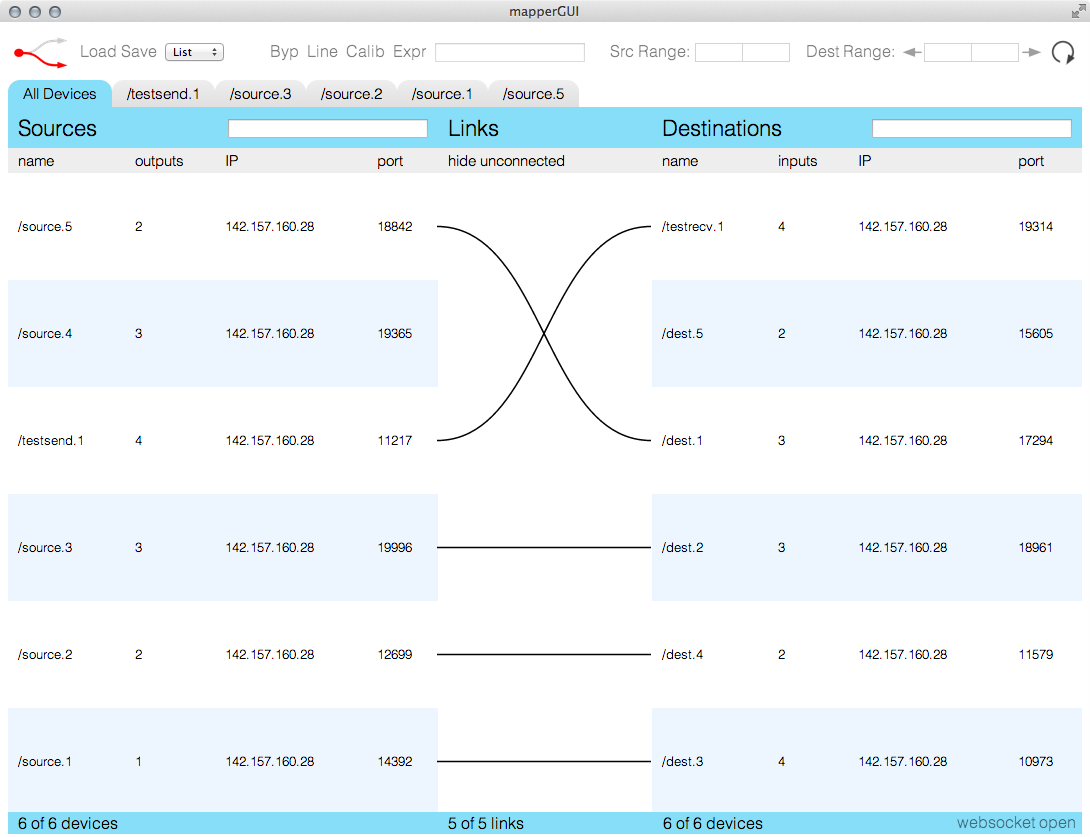
\includegraphics{figures/list_view_all_devices}}
\caption{The list view with all devices selected}
\label{fig:list_view_all_devices}
\end{figure}

The view itself is divided into two major modes: ``All Devices'' and individual linked source devices. Switching between these modes is accomplished through tabs that appear at the top of the container, much like the tabs that appear in modern web browsers. In the All Devices tab, every device displayed on the network is listed in one of the two columns, as in \ref{fig:list_view_all_devices}. Source devices are listed in the left table, while the right table lists destination devices. Intermediate devices, such as implicit mappers described in \cite{interpolated_mappings}, will be listed in both tables. Here arrows represent links between devices. Currently the GUI provides users with names, the number of child signals, IP addresses and a port for every device. Since no connections or signals are displayed, most of the top bar (see section \ref{sec:top_toolbar}) is disabled in the All Devices tab. Saving and loading are also disabled.

\begin{figure}[ht]
\centering
	\scalebox{0.4}{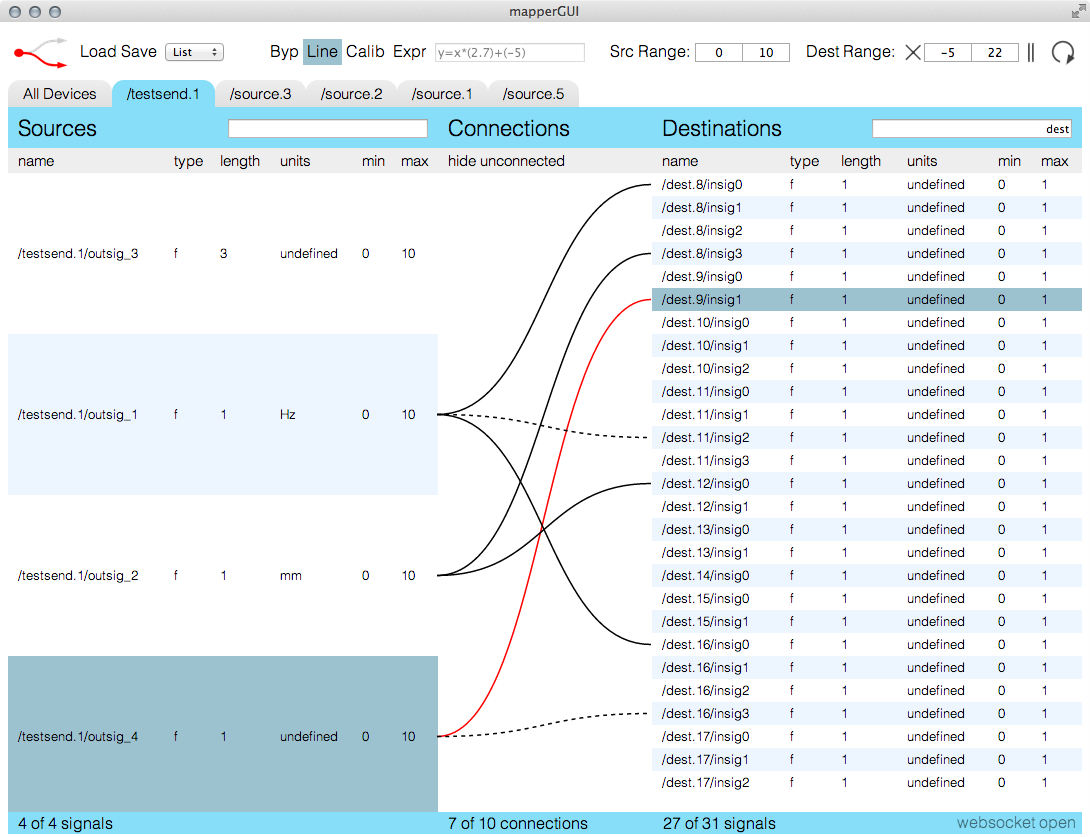
\includegraphics{figures/list_view_single_link}}
\caption{The list view with device \textbf{testsend.1} selected}
\label{fig:list_view_single_link}
\end{figure}

The GUI draws a tab for every source device with at least one link to a destination device. Clicking on any of these devices will redraw both tables. The left table now shows all child signals for the selected source device while the right table displays child signals for every destination device linked to the selected device. 

	% subsection the_list_view (end)
	
	\subsection{Display libmapper metadata} % (fold)
	\label{sub:display_libmapper_metadata}

The original webmapper interface tables listing devices and signals have no headers. Without these queues, only a small amount of metadata is provided (see figure \ref{fig:webmapper}):

\begin{table}
	\centering
	\Tcaption{Metadata available in webmapper vs list view}
	\label{tab:webmapper_list_view_metadata}
		\begin{tabular}{l  l  |  l l }
		\hline\hline
		\textbf{webmapper}&&\textbf{list view}\\
		Devices&Signals&Devices&Signals\\
		\hline
		name&name&name&name\\
		IP address&data type&IP address&data type\\
		port&vector length&port&vector length\\
		&&number of inputs&units\\
		&&number of outputs&maximum value\\
		&&&minimum value\\
		\end{tabular}
\end{table}

To include a necessary feature of max mapper, column headers are added to the list view. Also included are the new pieces of device and signal metadata listed in table \ref{tab:webmapper_list_view_metadata}. Tables draw themselves with invisible extra columns, such that adding extra data can be easily accomplished. If a user embeds extra metadata not listed above onto devices or signals, that data will automatically be included in the table display.  

In general, the GUI tries to keep possible extensions to libmapper like this in mind. Very little is assumed about the network itself. In turn, the only device metadata that \emph{must} exist is the name and number of inputs/outputs, which is used to either display the device as a source or destination. For signals, the GUI takes vector length into account when deciding whether two signals are compatible and can be connected. However, dis-including length in the signal metadata will not result in an error.
	
	% subsection display_libmapper_metadata (end)

	\subsection{Visual feedback} % (fold)
	\label{sub:visual_feedback}

Maxmapper 
		% # of signals/etc.
		% muted lines
		% row striping

	% subsection visual_feedback (end)

	\subsection{Namespace filtering} % (fold)
	\label{sub:namespace_filtering}
		%hide unconnected signals
	% subsection namespace_filtering (end)

	\subsection{Draggable connections and links} % (fold)
	\label{sub:draggable_connections_and_links}
	
	% subsection draggable_connections_and_links (end)

% section integration_of_interface_features (end)

%%%%%%%%%%%%%%%%%%%%%%%%%%%%%%%%%%%%%%%%%%%%%%%%%%%%%%%%%%%%%%%%%%%%%%%%%%%%%%%%%%%%%%%%%%%%%%%%%%%%%%%%%%%%%%%%%%%%%%%%%%%%%%%%%%%%%%%%%%%%%%%%%%%%%%%%%%%%%%%%%%%%%%%%%%%%%%%%%%%%%%%%%%%%%%%%%%%%%%%%%%%%%%%%%%%%%%%%%%%%%%%%%%%%%%%%%%%%%%%%%%%%%%%%%%%%%%%%%%
\section{Extension of Control and Visual Elements} % (fold)
\label{sec:extension_of_control_and_visual_elements}

	\subsection{Keyboard shortcuts} % (fold)
	\label{sec:keyboard_shortcuts}

		%select all, large selections
	
	% subsection keyboard_shortcuts (end)

	\subsection{Window resizing} % (fold)
	\label{sec:window_resizing}
	
	% subsection window_resizing (end)

	\subsection{Variable line heights} % (fold)
	\label{sec:variable_line_heights}
	
	% subsection variable_line_heights (end)

	\subsection{Visual Redesign} % (fold)
	\label{sec:visual_redesign}
	
	% subsection visual_redesign (end)

	\subsection{Grid \& Hive views} % (fold)
	\label{sec:grid_&_hive_views}

\begin{figure}[ht]
\centering
	\scalebox{0.4}{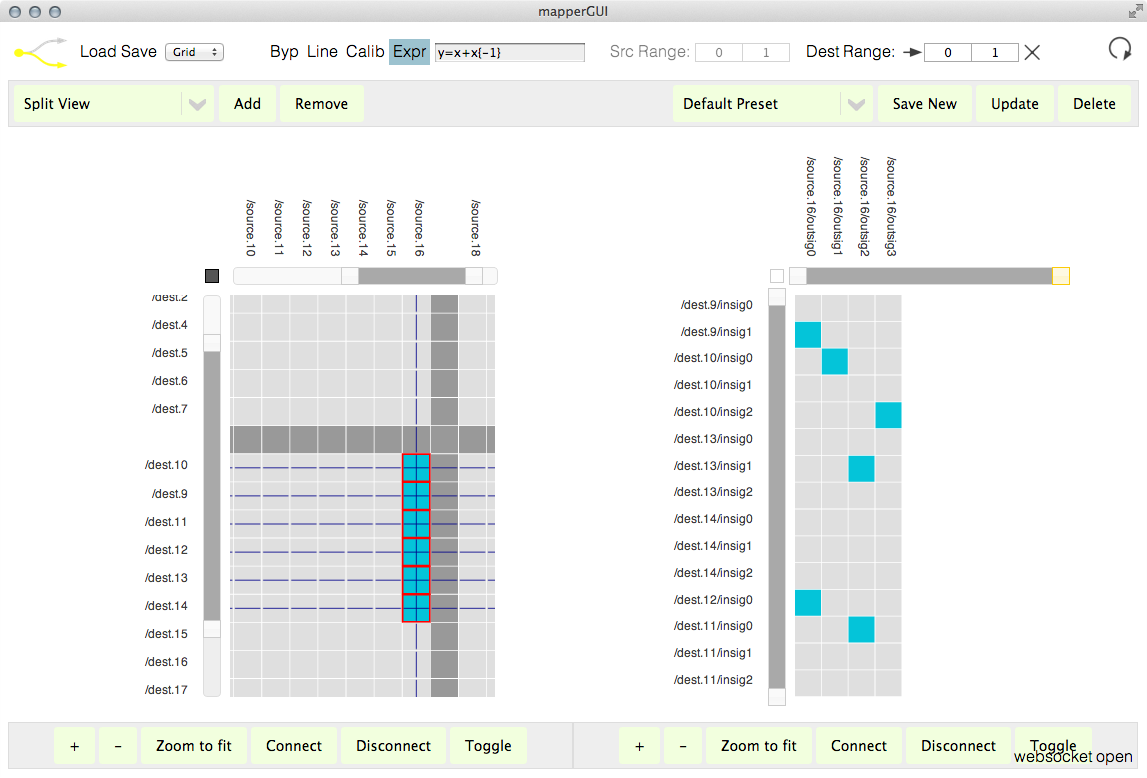
\includegraphics{figures/grid}}
\caption{The grid view}
\label{fig:grid}
\end{figure}

\begin{figure}[ht]
\centering
	\scalebox{0.4}{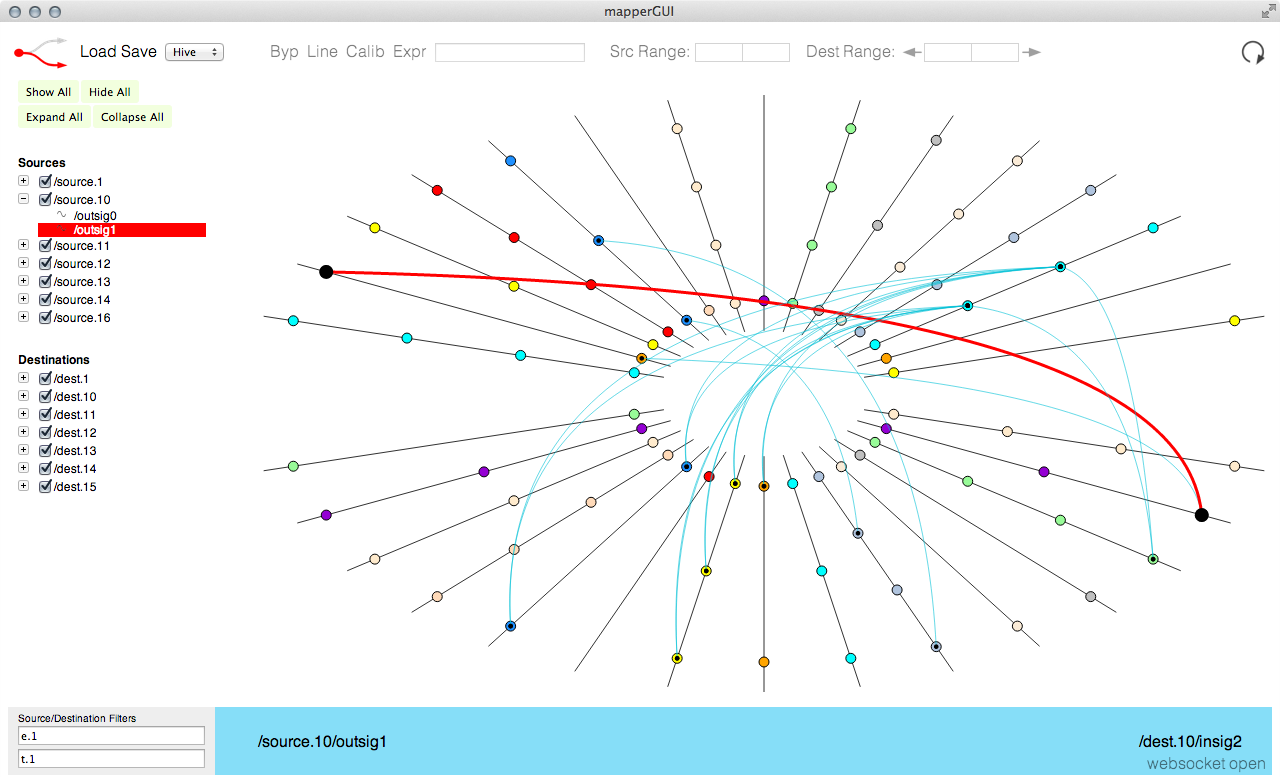
\includegraphics{figures/hive}}
\caption{The hive view}
\label{fig:hive}
\end{figure}
	
	% subsection grid_&_hive_views (end)

% section extension_of_control_and_visual_elements (end)

%%%%%%%%%%%%%%%%%%%%%%%%%%%%%%%%%%%%%%%%%%%%%%%%%%%%%%%%%%%%%%%%%%%%%%%%%%%%%%%%%%%%%%%%%%%%%%%%%%%%%%%%%%%%%%%%%%%%%%%%%%%%%%%%%%%%%%%%%%%%%%%%%%%%%%%%%%%%%%%%%%%%%%%%%%%%%%%%%%%%%%%%%%%%%%%%%%%%%%%%%%%%%%%%%%%%%%%%%%%%%%%%%%%%%%%%%%%%%%%%%%%%%%%%%%%%%%%%%%
\section{Other GUI features} % (fold)
\label{sec:other_gui_features}

	\subsection{Saving \& Loading} % (fold)
	\label{sec:saving_and_loading}
	
	% subsection saving_&_loading (end)

	\subsection{Creation of a standalone \& distribution} % (fold)
	\label{sec:creation_of_a_standalone_and_distribution}
	
	% subsection creation_of_a_standalone_&_distribution (end)

% section other_gui_features (end)




